\chapter{\EN{Task manager practical joke}\RU{Шутка с task manager} (Windows Vista)}
\index{Windows!Windows Vista}

\RU{У меня только 4 ядра в процессоре в компьютере, так что Task Manager в Windows показывает только 4
графика загрузки процессора.}
\EN{I have only 4 CPU cores on my computer, so the Windows Task Manager shows only 4 CPU load graphs.}

\RU{Посмотрим, сможем ли мы немного хакнуть Task Manager, чтобы он находил больше ядер в компьютере.}
\EN{Let's see if it's possible to hack Task Manager slightly so it would detect more CPU cores.}

\index{Windows!NTAPI}
\RU{В начале задумаемся, откуда Task Manager знает количество ядер?}
\EN{Let us first think, how does the Task Manager know the number of cores?}
\RU{В win32 имеется функция \TT{GetSystemInfo()}, при помощи которой можно узнать.}
\EN{There is the \TT{GetSystemInfo()} win32 function present in win32 userspace which can tell us this.}
\RU{Но она не импортируется в}\EN{But it's not imported in} \TT{taskmgr.exe}.
\RU{Есть еще одна в \gls{NTAPI}, \TT{NtQuerySystemInformation()}, которая используется в 
\TT{taskmgr.exe} в ряде мест.}
\EN{There is, however, another one in \gls{NTAPI}, \TT{NtQuerySystemInformation()}, 
which is used in \TT{taskmgr.exe} in several places.}
\RU{Чтобы узнать количество ядер, нужно вызвать эту функцию с константной \TT{SystemBasicInformation} в 
первом аргументе (а это ноль}
\EN{To get the number of cores, one has to call this function with the \TT{SystemBasicInformation} constant
as a first argument (which is zero}
\footnote{\href{http://go.yurichev.com/17251}{MSDN}}).

\RU{Второй аргумент должен указывать на буфер, который примет всю информацию.}
\EN{The second argument has to point to the buffer which is getting all the information.}

\RU{Так что нам нужно найти все вызовы функции \TT{NtQuerySystemInformation(0, ?, ?, ?)}.}
\EN{So we need to find all calls to the \TT{NtQuerySystemInformation(0, ?, ?, ?)} function.}
\RU{Откроем}\EN{Let's open} \TT{taskmgr.exe} \InENRU IDA. 
\index{Windows!PDB}
\RU{Что всегда хорошо с исполняемыми файлами от Microsoft, это то что IDA может скачать соответствующуий 
\gls{PDB}-файл именно для этого файла и добавить все имена функций.}
\EN{What is always good about Microsoft executables is that IDA can download the corresponding \gls{PDB} 
file for this executable and show all function names.}
\RU{Видимо, Task Manager написан на \Cpp и некоторые функции и классы имеют говорящие за себя имена.}
\EN{It is visible that Task Manager is written in \Cpp and some of the function names and classes are really 
speaking for themselves.}
\RU{Тут есть классы}\EN{There are classes} CAdapter, CNetPage, CPerfPage, CProcInfo, CProcPage, CSvcPage, 
CTaskPage, CUserPage.
\RU{Должно быть, каждый класс соответствует каждой вкладке в Task Manager.}
\EN{Apparently, each class corresponds to each tab in Task Manager.}

\RU{Я прошелся по всем вызовам и добавил комментарий с числом, передающимся как первый аргумент.}
\EN{I visited each call and added comment with tue value which is passed as the first function argument.}
\RU{В некоторых местах я написал ``not zero'', потому что значение в тех местах однозначно не ноль, 
но что-то другое (больше об этом во второй части главы).}
\EN{I wrote ``not zero'' at some places, because the value there was clearly not zero, 
but something really different (more about this in the second part of this chapter).}
\RU{А мы все-таки ищем ноль передаваемый как аргумент.}
\EN{And we are looking for zero passed as argument, after all.}

\begin{figure}[H]
\centering
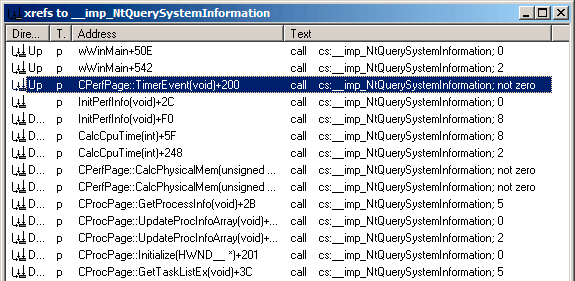
\includegraphics[scale=\FigScale]{examples/taskmgr/IDA_xrefs.png}
\caption{IDA: \RU{вызовы функции}\EN{cross references to} NtQuerySystemInformation()}
\end{figure}

\RU{Да, имена действительно говорящие сами за себя.}
\EN{Yes, the names are really speaking for themselves.}

\RU{Когда я внимательно изучил каждое место, где вызывается \TT{NtQuerySystemInformation(0, ?, ?, ?)},
я быстро нашел то что нужно в функции \TT{InitPerfInfo()}:}
\EN{When I closely investigated each place where \TT{NtQuerySystemInformation(0, ?, ?, ?)} is called,
I quickly found what I need in the \TT{InitPerfInfo()} function:}

\lstinputlisting[caption=taskmgr.exe (Windows Vista)]{examples/taskmgr/taskmgr.lst}

\TT{g\_cProcessors} \RU{это глобальная переменная и это имя присвоено IDA в соответствии с \gls{PDB}-файлом,
скачанным с сервера символов Microsoft}\EN{is a global variable, and this name was assigned by 
IDA according to the \gls{PDB} loaded from Microsoft's symbol server}.

\RU{Байт берется из}\EN{The byte is taken from} \TT{var\_C20}. 
\RU{И}\EN{And} \TT{var\_C58} \RU{передается в}\EN{is passed to} \TT{NtQuerySystemInformation()} 
\RU{как указатель на принимающий буфер}\EN{as a pointer to the receiving buffer}.
\RU{Разница между}\EN{The difference between} 0xC20 \AndENRU 0xC58 \RU{это}\EN{is} 0x38 (56).
\RU{Посмотрим на формат структуры, который можно найти в MSDN:}
\EN{Let's take a look at format of the return structure, which we can find in MSDN:}

\begin{lstlisting}
typedef struct _SYSTEM_BASIC_INFORMATION {
    BYTE Reserved1[24];
    PVOID Reserved2[4];
    CCHAR NumberOfProcessors;
} SYSTEM_BASIC_INFORMATION;
\end{lstlisting}

\RU{Это система x64, так что каждый PVOID занимает здесь 8 байт.}
\EN{This is a x64 system, so each PVOID takes 8 byte.}
\RU{Так что все \IT{reserved}-поля занимают $24+4*8=56$.}
\EN{All \IT{reserved} fields in the structure take $24+4*8=56$ bytes.}
\RU{О да, это значит, что \TT{var\_C20} в локальном стеке это именно поле
\TT{NumberOfProcessors} структуры \TT{SYSTEM\_BASIC\_INFORMATION}.}
\EN{Oh yes, this implies that \TT{var\_C20} is the local stack is exactly the
\TT{NumberOfProcessors} field of the \TT{SYSTEM\_BASIC\_INFORMATION} structure.}

\RU{Проверим, прав ли я}\EN{Let's check if I'm right}.
\RU{Скопируем}\EN{Copy} \TT{taskmgr.exe} \RU{из}\EN{from} \TT{C:\textbackslash{}Windows\textbackslash{}System32} 
\RU{в какую-нибудь другую папку}\EN{to some other folder} 
(\RU{чтобы}\EN{so the} \IT{Windows Resource Protection} \RU{не пыталась восстанавливать измененный}
\EN{will not try to restore the patched} \TT{taskmgr.exe}).

\RU{Откроем его в Hiew и найдем это место:}
\EN{Let's open it in Hiew and find the place:}

\begin{figure}[H]
\centering
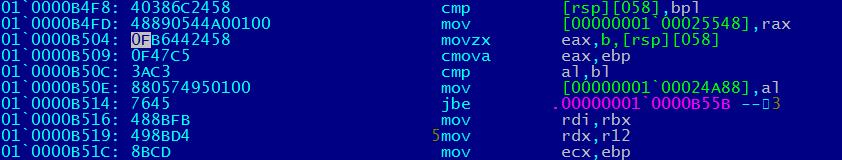
\includegraphics[scale=\FigScale]{examples/taskmgr/hiew2.png}
\caption{Hiew: \RU{найдем это место}\EN{find the place to be patched}}
\end{figure}

\RU{Заменим инструкцию \TT{MOVZX} на нашу.}
\EN{Let's replace the \TT{MOVZX} instruction with ours.}
\RU{Сделаем вид что у нас 64 ядра процессора}\EN{Let's pretend we've got 64 CPU cores}.
\RU{Добавим дополнительную инструкцию \ac{NOP} (потому что наша инструкция короче чем та что там сейчас):}
\EN{Add one additional \ac{NOP} (because our instruction is shorter than the original one):}

\begin{figure}[H]
\centering
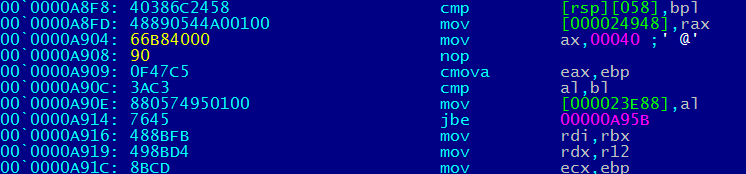
\includegraphics[scale=\FigScale]{examples/taskmgr/hiew1.png}
\caption{Hiew: \RU{меняем инструкцию}\EN{patch it}}
\end{figure}

\RU{И это работает}\EN{And it works}!
\RU{Конечно же, данные в графиках неправильные}\EN{Of course, the data in the graphs is not correct}.
\RU{Иногда, Task Manager даже показывает общую загрузку CPU более 100\%.}
\EN{At times, Task Manager even shows an overall CPU load of more than 100\%.}

\begin{figure}[H]
\centering
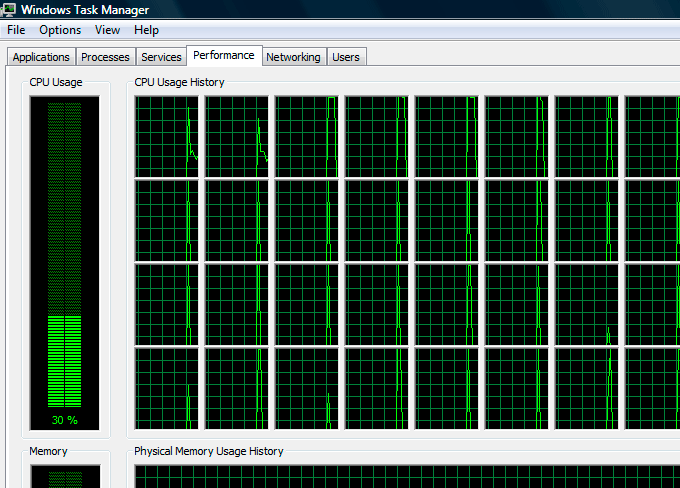
\includegraphics[scale=\FigScale]{examples/taskmgr/taskmgr_64cpu_crop.png}
\caption{\RU{Обманутый}\EN{Fooled} Windows Task Manager}
\end{figure}

\RU{Я выбрал число 64, потому что Task Manager падает если установить б\'{о}льшее значение.}
\EN{I picked the number 64, because Task Manager crashes if you try to set a larger value.}
\RU{Должно быть, Task Manager в Windows Vista не тестировался на компьютерах с большим количеством ядер.}
\EN{Apparently, Task Manager in Windows Vista was not tested on computers with a large number of cores.}
\RU{И, наверное, там есть внутри какие-то статичные структуры данных, ограниченные до 64-х ядер.}
\EN{So there are probably some static data structures inside it limited to 64 cores.}

\section{\RU{Использование LEA для загрузки значений}\EN{Using LEA to load values}}
\label{TaskMgr_LEA}

\RU{Иногда, \TT{LEA} используется в \TT{taskmgr.exe} вместо \TT{MOV} для установки первого аргумента 
\TT{NtQuerySystemInformation()}:}
\EN{Sometimes, \TT{LEA} is used in \TT{taskmgr.exe} instead of \TT{MOV} to set the first argument of 
\TT{NtQuerySystemInformation()}:}

\lstinputlisting[caption=taskmgr.exe (Windows Vista)]{examples/taskmgr/taskmgr2.lst}

\index{x86!\Instructions!LEA}
\RU{Честно говоря, я не знаю почему, но \ac{MSVC} часто так делает.}
\EN{I honestly, don't know why, but it is what \ac{MSVC} often does.}
\RU{Может быть, это какая-то оптимизация и \TT{LEA} работает быстрее или лучше, чем загрузка значения 
используя \TT{MOV}?}
\EN{Maybe this is some kind of optimization and \TT{LEA} works faster or better than loading
values using \TT{MOV}?}

\RU{Еще один пример подобного}\EN{Another example of such thing is}: 
\myref{using_MOV_and_pack_of_LEA_to_load_values}.
